%!TEX root = brainreader.tex

\section{Introduction}
\IEEEPARstart{F}{unctional} magnetic resonance imaging, or fMRI, data can shed light on what individuals are looking at.  Specific areas in the brain are known to react strongly to particular line orientations and locations.  Using activation data from these centers, such fMRI data can ``reconstruct'' what an individual is seeing.

The Gallant lab from UC Berkeley has worked on this problem previously, demonstrating \valkyrie{citation needed} that they can perform this reconstruction by averaging images from a training set.  The top 100 images whose recorded fMRI profiles match most closely with the recorded data are simply stacked on top of each other to create output videos.

However, this type of visualization is very ``messy'': while the quantified fMRI matches are quite strong, the visual output video stacks are misleadingly inaccurate.  Using computational techniques, we can improve the quality of these output videos (Figure \ref{fig:avg})


\begin{figure}[t]
\centering
    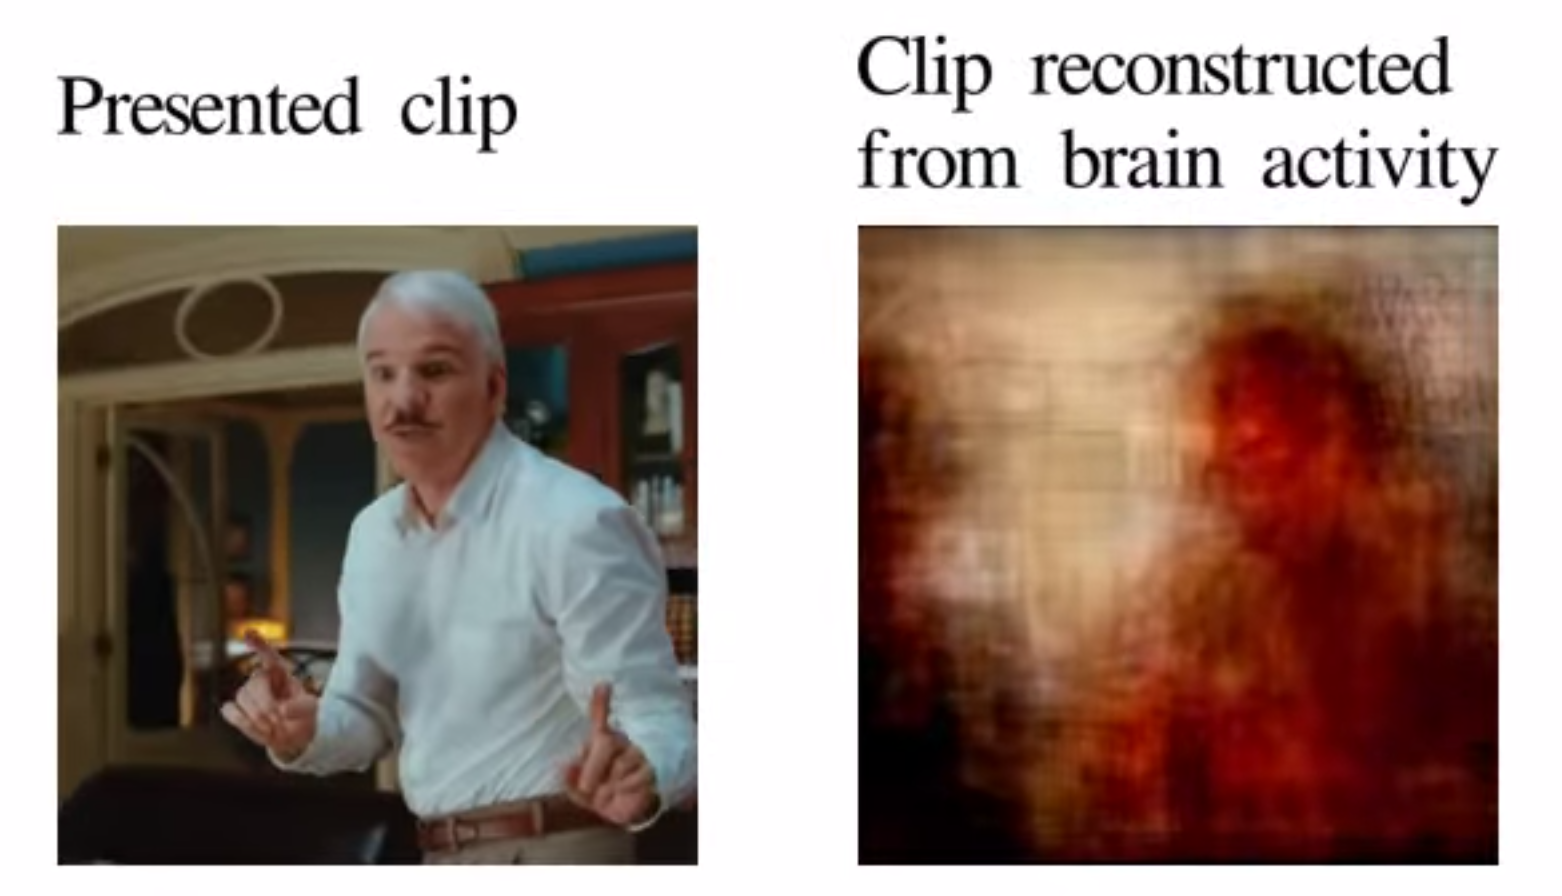
\includegraphics[width=1.0\columnwidth]{figures/average.png}
\caption{a) The first generation of visualization for BrainReader clips: the top 100 guesses are simply averaged and overlaid to create an output image at each frame.  This belies the accuracy of the technique, which is quite high. b) Our improved visualization \valkyrie{obviously need image here.}.}
\label{fig:avg}
\end{figure}


Instead of a simple averaging process for turning guesses into an output video, we used several more sophisticated approaches.  First, we simply performed weighted averaging, using clip ranking as our weights.  This already constituted an improvement over na\"{i}ve weighting (Figure \ref{fig:weighted}).

\begin{figure}[t]
\centering
    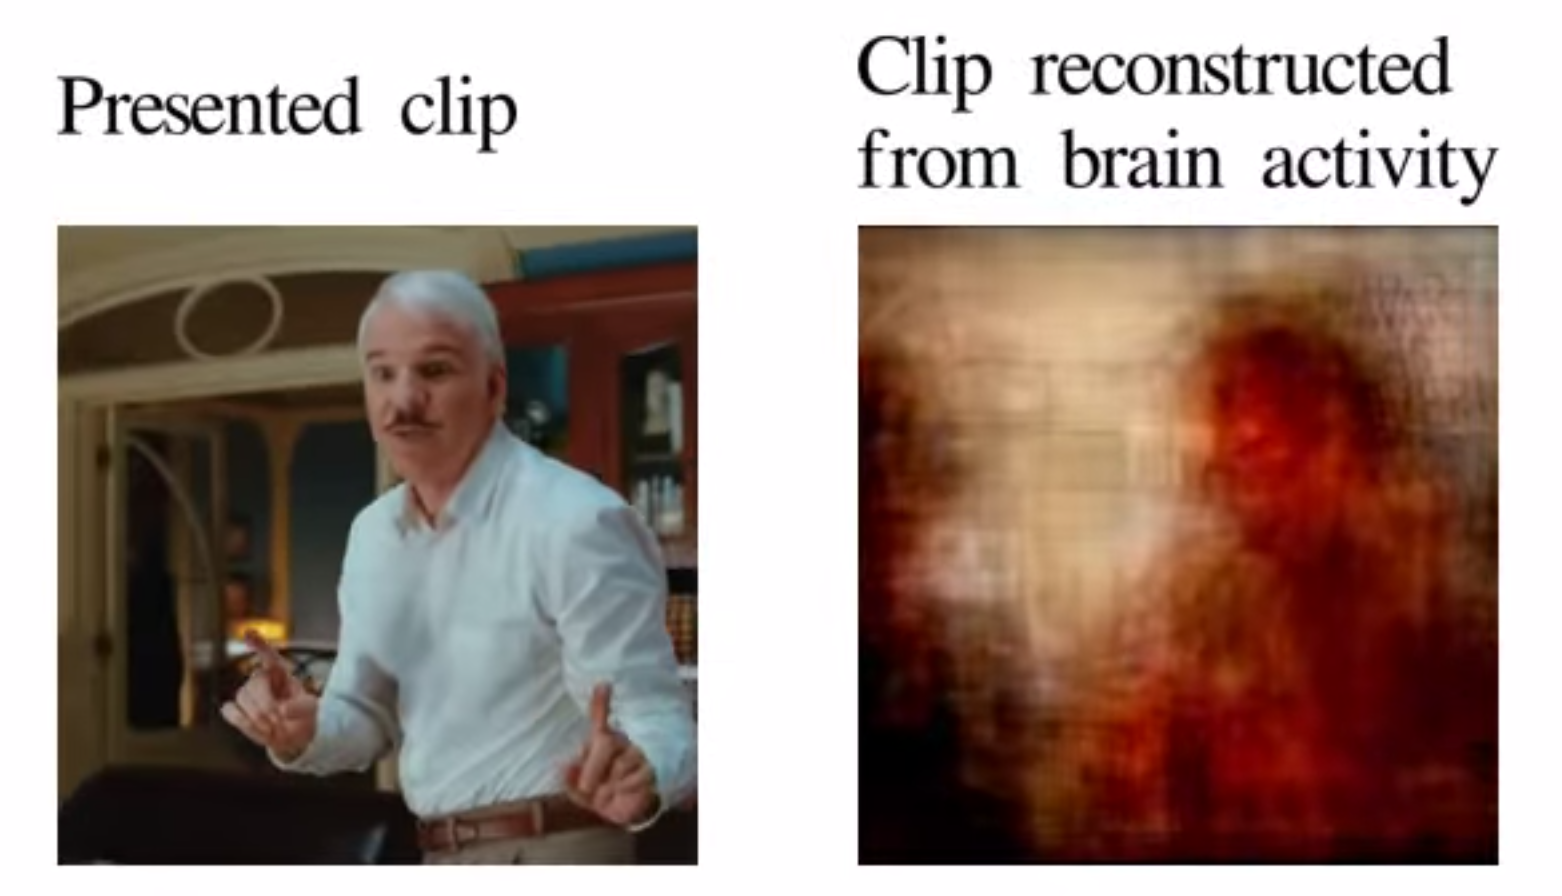
\includegraphics[width=1.0\columnwidth]{figures/average.png}
\caption{Using a weighted average improves over the na\"{i}ve average seen in Figure \ref{fig:avg}a. \valkyrie{obviously we need this image as well.}}
\label{fig:weighted}
\end{figure}


After using weighted averaging, we turned to even more sophisticated techniques: HOG feature alignment and SIFT flow.  These give us additional information on the edges makeup and semantic scene composition of both the original clip and the top 100 guesses as predicted by the original fMRI-based system.